\subsection{Die Amplitude und Phasenverschiebung der Kondensatorspannung}
Im zweiten Teil des Versuchs wird die Amplitude $A$ der Kondensatorspannung und die Phasenverschiebung $\phi$ zwischen Generator-
und Kondensatorspannung eines RC-Gliedes bei angeschlossener Sinusspannung in Abhängigkeit der Frequenz untersucht.
Hierfür wird ein Zweikanal-Oszillograph wie er in Abbildung \ref{fig:ampl_phasenverschiebung} zu sehen ist angeschlossen.
Das Triggersignal beider Kanäle wird AC gekoppelt.
Der Kondensator wird an Kanal 1 und der Generator an Kanal 2 angeschlossen.
\begin{figure}[H]
    \centering
    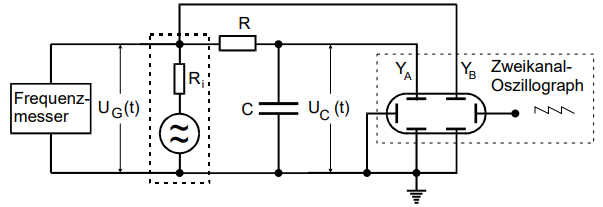
\includegraphics[height=5cm]{abbildungen/ampl_phasenverschiebung.png}
    \caption{Schaltung zur Messung der Amplitude und Phasenverschiebung \cite{man:v353}.}
    \label{fig:ampl_phasenverschiebung}
\end{figure}
\noindent
Es werden mehrere Frequenzen $f$ zwischen ca. \qty{0}{\hertz} und \qty{1000}{\hertz} eingestellt.
Dabei müssen je nach Größenordnung die Regler Timediv und Voltdiv angepasst werden.
Zum leichteren Ablesen der einzelnen Werte können die Graphen erneut mittels des x-Positionsreglers verschoben werden.
Generell ist darauf zu achten, dass beide Graphen symmetrisch zur x-Achse liegen.
Am Oszilloskop ergibt sich in etwa ein Graph wie in Abbildung \ref{fig:graph_phasenverschiebung}.
\begin{figure}[H]
    \centering
    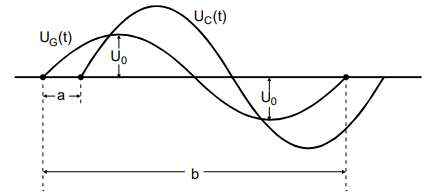
\includegraphics[height=3cm]{abbildungen/graph_phasenverschiebung.png}
    \caption{Darstellung zur Bestimmung von $\phi$ \cite{man:v353}.}
    \label{fig:graph_phasenverschiebung}
\end{figure}
\noindent
Es wird festgestellt, dass die Amplitude der Generatorspannung einen konstanten Wert $U_0 = \qty[]{1.55}{\volt}$ unabhänig von $f$ hat.
Die Amplitude der Kondensatorspannung $A$ kann sofort abgelesen werden.
Zur Bestimmung der Phasenverschiebung $\phi$ muss zunächst der zeitliche Abstand $a = \Delta t$ der beiden Nulldurchgänge bestimmt werden.
Die Schwingungsdauer $b$ lässt sich mittels $b = \frac{1}{f}$ ermitteln.
Somit ergibt sich 
\begin{align}
    \phi = 2 \pi \, \frac{a}{b}.
    \label{eq:phase}
\end{align}
%